\documentclass[class=article,border=0pt]{standalone}
\usepackage[dvipsnames]{xcolor}
\usepackage{fancybox,pstricks,pst-node,tikz,times}

\newcommand*{\xMin}{0}%
\newcommand*{\xMax}{8}%
\newcommand*{\yMin}{0}%
\newcommand*{\yMax}{6}%
\begin{document}

\pagestyle{empty}%
\thispagestyle{empty}%
\psset{linewidth=1.5pt,framearc=0.3}%
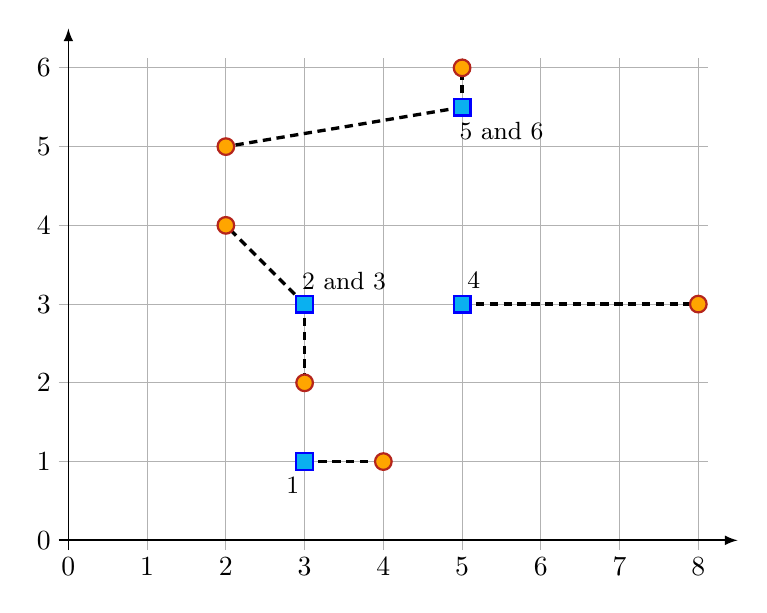
\begin{tikzpicture}

% Grid
\foreach \i in {\xMin,...,\xMax} {
  \draw [draw=none] (\i,\yMin) -- (\i,\yMax)  node [below] at (\i,\yMin-0.1) {$\i$};
}
\foreach \i in {\yMin,...,\yMax} {
   \draw [draw=none] (\xMin,\i) -- (\xMax,\i) node [left] at (\xMin-0.1,\i) {$\i$};
}
\draw[step=10mm, line width=0.1mm, black!30]
  (\xMin-0.125,\yMin-0.125) grid (\xMax+0.125,\yMax+0.125);
\draw [semithick, ->, >=latex] (0,\yMin-0.125)--(0,\yMax+0.5);
\draw [semithick, ->, >=latex] (\xMin-0.125,0)--(\xMax+0.5, 0);

\def \apfill {Orange}
\def \apdraw {BrickRed}

\def \teamfill {ProcessBlue}
\def \teamdraw {Blue}

% Wires and team/AP markers
\draw [densely dashed,very thick] (3,1) -- (4,1);
\filldraw[draw=\teamdraw,fill=\teamfill,thick] (3,1) + (-3.0pt,-3.0pt) rectangle +(3.0pt,3.0pt);
\filldraw[draw=\apdraw,fill=\apfill, thick] (4,1) circle (3.0pt);

\draw [densely dashed,very thick] (3,3) -- (2,4);
\filldraw[draw=\teamdraw,fill=\teamfill,thick] (3,3) + (-3.0pt,-3.0pt) rectangle +(3.0pt,3.0pt);
\filldraw[draw=\apdraw,fill=\apfill, thick] (2,4) circle (3.0pt);

\draw [densely dashed,very thick] (3,3) -- (3,2);
\filldraw[draw=\teamdraw,fill=\teamfill,thick] (3,3) + (-3.0pt,-3.0pt) rectangle +(3.0pt,3.0pt);
\filldraw[draw=\apdraw,fill=\apfill, thick] (3,2) circle (3.0pt);

\draw [densely dashed,very thick] (5,3) -- (8,3);
\filldraw[draw=\teamdraw,fill=\teamfill,thick] (5,3) + (-3.0pt,-3.0pt) rectangle +(3.0pt,3.0pt);
\filldraw[draw=\apdraw,fill=\apfill, thick] (8,3) circle (3.0pt);

\draw [densely dashed,very thick] (5,5.5) -- (5,6);
\filldraw[draw=\teamdraw,fill=\teamfill,thick] (5,5.5) + (-3.0pt,-3.0pt) rectangle +(3.0pt,3.0pt);
\filldraw[draw=\apdraw,fill=\apfill, thick] (5,6) circle (3.0pt);

\draw [densely dashed,very thick] (5,5.5) -- (2,5);
\filldraw[draw=\teamdraw,fill=\teamfill,thick] (5,5.5) + (-3.0pt,-3.0pt) rectangle +(3.0pt,3.0pt);
\filldraw[draw=\apdraw,fill=\apfill, thick] (2,5) circle (3.0pt);

\node at (2.85,0.70) {\small $1$};
\node at (3.50,3.30) {\small $2$ and $3$};
\node at (5.15,3.30) {\small $4$};
\node at (5.50,5.20) {\small $5$ and $6$};

\end{tikzpicture}


\end{document}
